% Created by tikzDevice version 0.12.3.1 on 2021-04-14 21:08:27
% !TEX encoding = UTF-8 Unicode
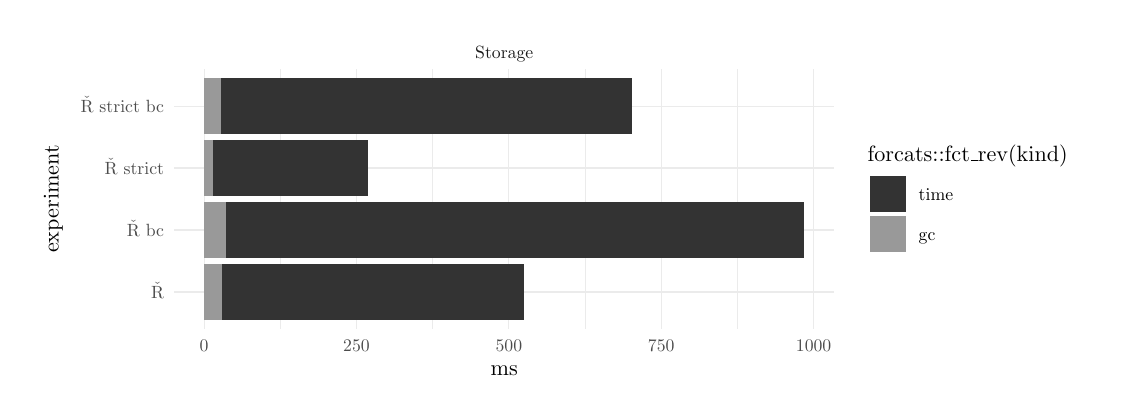
\begin{tikzpicture}[x=1pt,y=1pt]
\definecolor{fillColor}{RGB}{255,255,255}
\path[use as bounding box,fill=fillColor,fill opacity=0.00] (0,0) rectangle (390.26,130.09);
\begin{scope}
\path[clip] ( 52.89, 21.16) rectangle (291.52,115.19);
\definecolor{drawColor}{gray}{0.92}

\path[draw=drawColor,line width= 0.2pt,line join=round] ( 91.27, 21.16) --
	( 91.27,115.19);

\path[draw=drawColor,line width= 0.2pt,line join=round] (146.34, 21.16) --
	(146.34,115.19);

\path[draw=drawColor,line width= 0.2pt,line join=round] (201.41, 21.16) --
	(201.41,115.19);

\path[draw=drawColor,line width= 0.2pt,line join=round] (256.48, 21.16) --
	(256.48,115.19);

\path[draw=drawColor,line width= 0.4pt,line join=round] ( 52.89, 34.59) --
	(291.52, 34.59);

\path[draw=drawColor,line width= 0.4pt,line join=round] ( 52.89, 56.98) --
	(291.52, 56.98);

\path[draw=drawColor,line width= 0.4pt,line join=round] ( 52.89, 79.37) --
	(291.52, 79.37);

\path[draw=drawColor,line width= 0.4pt,line join=round] ( 52.89,101.76) --
	(291.52,101.76);

\path[draw=drawColor,line width= 0.4pt,line join=round] ( 63.74, 21.16) --
	( 63.74,115.19);

\path[draw=drawColor,line width= 0.4pt,line join=round] (118.80, 21.16) --
	(118.80,115.19);

\path[draw=drawColor,line width= 0.4pt,line join=round] (173.87, 21.16) --
	(173.87,115.19);

\path[draw=drawColor,line width= 0.4pt,line join=round] (228.94, 21.16) --
	(228.94,115.19);

\path[draw=drawColor,line width= 0.4pt,line join=round] (284.01, 21.16) --
	(284.01,115.19);
\definecolor{fillColor}{gray}{0.20}

\path[fill=fillColor] ( 70.28, 24.52) rectangle (179.26, 44.67);

\path[fill=fillColor] ( 67.02, 69.29) rectangle (122.98, 89.44);

\path[fill=fillColor] ( 71.64, 46.91) rectangle (280.67, 67.06);

\path[fill=fillColor] ( 69.77, 91.68) rectangle (218.30,111.83);
\definecolor{fillColor}{gray}{0.60}

\path[fill=fillColor] ( 63.74, 69.29) rectangle ( 67.02, 89.44);

\path[fill=fillColor] ( 63.74, 24.52) rectangle ( 70.28, 44.67);

\path[fill=fillColor] ( 63.74, 46.91) rectangle ( 71.64, 67.06);

\path[fill=fillColor] ( 63.74, 91.68) rectangle ( 69.77,111.83);
\end{scope}
\begin{scope}
\path[clip] ( 52.89,115.19) rectangle (291.52,127.24);
\definecolor{drawColor}{gray}{0.10}

\node[text=drawColor,anchor=base,inner sep=0pt, outer sep=0pt, scale=  0.64] at (172.20,119.01) {Storage};
\end{scope}
\begin{scope}
\path[clip] (  0.00,  0.00) rectangle (390.26,130.09);
\definecolor{drawColor}{gray}{0.30}

\node[text=drawColor,anchor=base,inner sep=0pt, outer sep=0pt, scale=  0.64] at ( 63.74, 13.15) {0};

\node[text=drawColor,anchor=base,inner sep=0pt, outer sep=0pt, scale=  0.64] at (118.80, 13.15) {250};

\node[text=drawColor,anchor=base,inner sep=0pt, outer sep=0pt, scale=  0.64] at (173.87, 13.15) {500};

\node[text=drawColor,anchor=base,inner sep=0pt, outer sep=0pt, scale=  0.64] at (228.94, 13.15) {750};

\node[text=drawColor,anchor=base,inner sep=0pt, outer sep=0pt, scale=  0.64] at (284.01, 13.15) {1000};
\end{scope}
\begin{scope}
\path[clip] (  0.00,  0.00) rectangle (390.26,130.09);
\definecolor{drawColor}{gray}{0.30}

\node[text=drawColor,anchor=base east,inner sep=0pt, outer sep=0pt, scale=  0.64] at ( 49.29, 32.39) {Ř};

\node[text=drawColor,anchor=base east,inner sep=0pt, outer sep=0pt, scale=  0.64] at ( 49.29, 54.78) {Ř bc};

\node[text=drawColor,anchor=base east,inner sep=0pt, outer sep=0pt, scale=  0.64] at ( 49.29, 77.17) {Ř strict};

\node[text=drawColor,anchor=base east,inner sep=0pt, outer sep=0pt, scale=  0.64] at ( 49.29, 99.55) {Ř strict bc};
\end{scope}
\begin{scope}
\path[clip] (  0.00,  0.00) rectangle (390.26,130.09);
\definecolor{drawColor}{RGB}{0,0,0}

\node[text=drawColor,anchor=base,inner sep=0pt, outer sep=0pt, scale=  0.80] at (172.20,  4.40) {ms};
\end{scope}
\begin{scope}
\path[clip] (  0.00,  0.00) rectangle (390.26,130.09);
\definecolor{drawColor}{RGB}{0,0,0}

\node[text=drawColor,rotate= 90.00,anchor=base,inner sep=0pt, outer sep=0pt, scale=  0.80] at ( 11.20, 68.18) {experiment};
\end{scope}
\begin{scope}
\path[clip] (  0.00,  0.00) rectangle (390.26,130.09);
\definecolor{drawColor}{RGB}{0,0,0}

\node[text=drawColor,anchor=base west,inner sep=0pt, outer sep=0pt, scale=  0.80] at (303.52, 81.87) {forcats::fct{\_{}}rev(kind)};
\end{scope}
\begin{scope}
\path[clip] (  0.00,  0.00) rectangle (390.26,130.09);
\definecolor{fillColor}{gray}{0.20}

\path[fill=fillColor] (304.23, 63.35) rectangle (317.26, 76.39);
\end{scope}
\begin{scope}
\path[clip] (  0.00,  0.00) rectangle (390.26,130.09);
\definecolor{fillColor}{gray}{0.60}

\path[fill=fillColor] (304.23, 48.90) rectangle (317.26, 61.93);
\end{scope}
\begin{scope}
\path[clip] (  0.00,  0.00) rectangle (390.26,130.09);
\definecolor{drawColor}{RGB}{0,0,0}

\node[text=drawColor,anchor=base west,inner sep=0pt, outer sep=0pt, scale=  0.64] at (321.97, 67.67) {time};
\end{scope}
\begin{scope}
\path[clip] (  0.00,  0.00) rectangle (390.26,130.09);
\definecolor{drawColor}{RGB}{0,0,0}

\node[text=drawColor,anchor=base west,inner sep=0pt, outer sep=0pt, scale=  0.64] at (321.97, 53.21) {gc};
\end{scope}
\end{tikzpicture}
